% TELFOR 2026, IEEE conference paper (A4, two-column, four-page limit).
% Build (from paper/):  tectonic telfor_revised.tex
%   (tectonic runs TeX -> BibTeX -> TeX as needed; with TeX Live instead:
%    pdflatex -> bibtex -> pdflatex x2.)
% Needs refs.bib and figures/evaluation_choices_revised.pdf, which is generated
% from the frozen JSON summaries by scripts/generate_telfor_revised_figure.py
% (hashes in figures/evaluation_choices_revised_manifest.json).
% The IEEE copyright notice is inserted by TELFOR for IEEE Xplore; keep the
% \IEEEpubid lines commented unless the camera-ready instructions say otherwise.

\documentclass[conference,a4paper]{IEEEtran}
\usepackage[utf8]{inputenc}
\usepackage[T1]{fontenc}
\usepackage{graphicx}
\usepackage{booktabs}
\usepackage{array}
\usepackage{amsmath}
\setlength{\textfloatsep}{6pt plus 2pt minus 3pt}
\setlength{\dbltextfloatsep}{6pt plus 2pt minus 3pt}
\setlength{\floatsep}{6pt plus 2pt minus 2pt}
\setlength{\abovecaptionskip}{3pt}

% \IEEEoverridecommandlockouts
% \IEEEpubid{\makebox[\columnwidth]{XXX-X-XXXX-XXXX-X/26/\$31.00~\copyright2026 IEEE \hfill}}

\begin{document}

\title{From IR Gains to Code-Size Savings:\\
Auditing LLVM Phase-Ordering Evaluation}

\author{\IEEEauthorblockN{Dimitrije Pe\v{s}i\'c}
\IEEEauthorblockA{\textit{School of Electrical Engineering, University of Belgrade}\\
Belgrade, Serbia\\
pd230014d@student.etf.bg.ac.rs}}

\maketitle

\begin{abstract}
Learned compiler pass ordering for code size is commonly scored by LLVM
instruction count against the \texttt{-Oz} pipeline. We ask how much of
such a result depends on three evaluation choices: how the reference is
prepared, which metric selects the candidate, and how binary size is
defined. We audit an existing experiment in the original CompilerGym
LLVM~10 service without retraining. On 120 NPB modules, giving the
reference and the candidates the size attributes that a source build
would carry reduces a fixed portfolio's instruction-count gain from
23.84\% to 0.08\%, while a 5.76\% code-section saving remains. A
service-faithful intervention attributes the gap to one transformation:
disabling loop unrolling removes 12,560 of the 12,639 excess
instructions of the plain reference. On 347 programs, selecting among
the same eight candidates by measured code bytes instead of instruction
count raises the saving for a graph-neural policy and for random search
alike, to 2.84--3.66\% and 2.82--3.68\%, with no consistent advantage
for the learned policy; a broader object-size metric ranks the results
differently. We recommend matched references, selection on the reported
metric, and explicitly defined size metrics.
\end{abstract}

\begin{IEEEkeywords}
compiler optimization, LLVM, phase ordering, code size, reinforcement
learning, evaluation methodology
\end{IEEEkeywords}

\section{Introduction}
A compiler lowers a program to an intermediate representation (IR),
transforms it with a sequence of optimization passes, and only then
generates machine code. Work on learned pass ordering usually scores a
pass sequence by the number of IR instructions it leaves, the
\emph{instruction count} (IC), because IC is cheap to compute and
independent of the target. IC is nevertheless a proxy. What is
deployed is bytes of machine code, and the code generator that produces
them makes its own size decisions: instruction selection, encodings,
alignment padding and duplicated loop tests change the byte count of
unchanged IR. Two modules with equal IC can therefore differ in size,
and a lower IC does not guarantee smaller code.

Choosing a pass order per program, the \emph{phase-ordering problem},
is undecidable in general~\cite{touati2006} and exhaustively searchable
only with heavy pruning~\cite{kulkarni2006}. A line of work therefore
learns program-specific orderings with reinforcement
learning~\cite{autophase,compilergym,posetrl,coreset,mammadli} and
reports gains over a fixed pipeline such as LLVM's \texttt{-Oz}. Such a
gain rests on three decisions that are seldom reported together: how
the reference pipeline's input is prepared, which metric picks the
winner among the candidates of a search, and which quantity is called
binary size.

This paper measures how far each decision moves the conclusion of one
existing experiment, a graph-neural-network (GNN) policy and its
random-search control in CompilerGym~\cite{compilergym}. We keep the
original service, action space, policy checkpoints and candidate budget
fixed and change only the evaluation. The contributions are: (1)~a
paired audit of reference preparation with a service-faithful causal
decomposition, which traces a large IC gain on the NPB suite to loop
unrolling in the reference; (2)~a generator-by-selector comparison that
measures all candidates of learned and random search under both
metrics; and (3)~evidence that two object-size definitions rank the
same candidates differently, with a small source-build control that
delimits the practical claim.

We do not propose a new optimizer, and the results are not evidence
that learned policies fail. Size attributes, fixed sequence portfolios
and selection by measured bytes are established tools; the contribution
is the controlled comparison and the causal decomposition. We examined
one protocol and make no claim about the references used in other
studies.

\section{Related Work}
AutoPhase~\cite{autophase} applied deep reinforcement learning to phase
ordering over a static feature vector, and CompilerGym~\cite{compilergym}
standardized the environments used here; it exposes both IC and
object-size observations, so a byte metric is not new. ProGraML~\cite{programl}
motivated graph representations of programs. POSET-RL~\cite{posetrl}
and the coreset approach of Liang et al.~\cite{coreset} restrict the
search to a small set of pass sequences or sub-sequences from which a
learned model chooses; a fixed portfolio is thus an existing idea. MLGO~\cite{mlgo} trains
an inlining policy directly against native size, and large language
models have been applied at a far larger budget~\cite{llmcompiler}.
Cummins et al.~\cite{compilergym} report that plain random search is
competitive with several autotuners, and Mammadli et al.~\cite{mammadli} find a learned
policy inferior to \texttt{-O3} on held-out programs. That LLVM's size
attributes steer optimization is documented compiler behaviour. Our
study is complementary to these works: it quantifies what reference
preparation and the selection metric contribute to a reported gain.

\section{Protocol}
\textbf{Environment and references.} All measurements run in the
unmodified CompilerGym~0.2.5 service with its bundled LLVM~10. The
reference is the service's own \texttt{-Oz} baseline path, and its
exported IC must equal the environment's \texttt{-Oz} observation.
Command-line \texttt{opt -Oz} builds a different pipeline and is never
used as the reference. We compare three preparations of the same
canonical module. \emph{P} (plain) is the module as the environment
provides it. \emph{A} (attributed) adds the function attributes
\texttt{minsize} and \texttt{optsize}, which \texttt{clang -Oz} attaches
to every function definition, and keeps the target triple and data
layout. \emph{U} is the plain module with
\texttt{llvm.loop.unroll.disable} added to every natural loop, existing
loop properties kept; the service has no unrolling switch, so the
intervention is made at the input and the service itself is unchanged.
Table~\ref{tab:prep} summarizes the preparations and what each one
isolates. In each condition the reference and all candidates start from
the same prepared module. A small LLVM~10 replica of the service's pass-manager
construction reproduces the service's output IR on every audited input;
we use it only to read LLVM's unrolling remarks, never as a reference.

\begin{table}[t]
\caption{Preparations of the same canonical module. The service and
its \texttt{-Oz} baseline path are identical in every row.}
\label{tab:prep}
\centering
\footnotesize
\setlength{\tabcolsep}{3pt}
\begin{tabular}{@{}l>{\raggedright\arraybackslash}p{0.53\columnwidth}>{\raggedright\arraybackslash}p{0.30\columnwidth}@{}}
\toprule
 & Input given to the service & Isolates \\
\midrule
P & module as provided, no size attributes & original reference \\
U & P + \texttt{llvm.loop.unroll.disable} on every loop & loop unrolling
alone \\
A & P + \texttt{minsize optsize} on every function definition & all
effects of the attributes \\
U$^{+}$ & optimized output of U + attributes, then \texttt{llc} only &
code generation on fixed IR \\
\bottomrule
\end{tabular}
\end{table}

\textbf{Cohorts.} Three cohorts support different comparisons and are
not pooled. The \emph{portfolio audit} covers 210 modules (120 NPB, 40
MiBench~\cite{mibench}, 50 BLAS) under P and A with eight pass sequences
fixed before the audit; the \emph{causal audit} is run on its 120 NPB
modules under P, U and A. The \emph{selector audit} covers 347 programs
(the same 210 plus 12 CHStone~\cite{chstone}, 28 csmith~\cite{csmith}
and 97 POJ-104) under A only. The \emph{source control} covers the 12
CHStone programs compiled from C source.

\textbf{Candidates and selection.} Each generator proposes eight
sequences of 45 actions from the same 36-pass action space. The learned
generator is a GNN policy from our earlier experiment, with three
checkpoints (training seeds 42, 123, 456); the eight episodes each
checkpoint sampled per program on the attributed input were recorded,
and we replay those action traces so that every candidate is measured.
Random search has five fixed realizations of eight uniformly drawn
sequences. Realizations are evaluated separately and never merged into
a larger budget. Two selectors act on the identical eight candidates:
minimum IC (the original rule) and minimum code-section bytes, the first
candidate winning ties. Selecting on the metric that is reported is
expected to help and is not a new algorithm; the empirical questions
are how much IC selection loses and whether the generators' ranking
changes.

\textbf{Metrics.} For every reference and candidate we record IC and
two sizes of the relocatable x86-64 object emitted by the bundled
\texttt{llc}: \emph{code-section bytes}, the sum of the \texttt{.text}
sections, and \emph{Berkeley text}, the \texttt{text} column of
\texttt{llvm-size}, which also counts other read-only allocated sections
such as constant data and unwind tables. Both are object-file
quantities, not the footprint of a linked binary. A gain is
$100\,(\sum \text{ref} - \sum \text{cand})/\sum \text{ref}$ over the
stated cohort, a ratio of sums that weights large modules more; it is
not a mean of per-program percentages. Ranges are the minimum and
maximum over checkpoints or realizations, not confidence intervals.

\begin{figure*}[t]
\centering
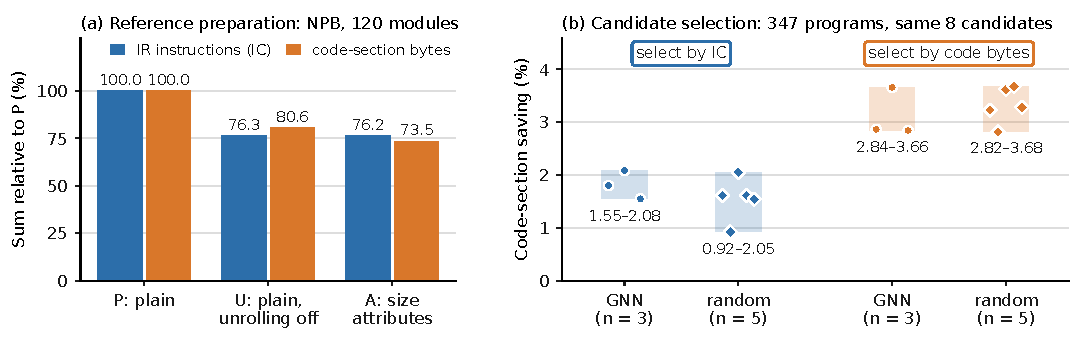
\includegraphics[width=\textwidth]{figures/evaluation_choices_revised.pdf}
\caption{Two evaluation choices in the original CompilerGym LLVM~10
service. (a)~Service \texttt{-Oz} reference on 120 NPB modules under
three input preparations, each metric summed and indexed to the plain
reference P (absolute sums in Table~\ref{tab:causal}). (b)~Code-section
saving over the attributed service \texttt{-Oz}, summed over 347
programs, when the winner among the same eight candidates is chosen by
IC or by code bytes. Each point is one GNN checkpoint or one
random-search realization; bands and labels give the minimum and
maximum, not a confidence interval.}
\label{fig:choices}
\end{figure*}

\section{Results}

\subsection{Reference preparation changes the verdict}
In the portfolio audit the candidate is chosen by IC. On the 120 NPB
modules, the portfolio's IC gain over the service \texttt{-Oz} is
23.84\% under P and 0.08\% under A; its code-section gain is 23.71\%
under P and 5.76\% under A. Aligning the attributes thus removes almost
the entire IC advantage but not the entire byte advantage, so the IC
result predicts neither the size nor the persistence of the
code-section result. The change is specific to the suite; MiBench and
BLAS move far less (per-suite tables are in the repository).

\subsection{Loop unrolling explains the NPB instruction-count gap}
The paired audit shows that the attributes matter, not which
transformation reads them. Loop unrolling is the natural suspect: it
replaces a loop by copies of its body, trading size for speed, and a
size build is expected to suppress it. Table~\ref{tab:causal} and
Fig.~\ref{fig:choices}(a) give the service reference under the three
preparations. The service requests a size-oriented pipeline in both
conditions, yet with plain input that pipeline still fully unrolls
constant-trip-count loops: LLVM reports 449 unrolling remarks on 43 of
the 120 modules, and none with the attributes. The pipeline-level
setting alone did not stop unrolling; the function attributes did.
Disabling unrolling alone removes 12,560 of the 12,639 IC by which P
exceeds A. On each of the 43 modules, U has exactly the IC of A and the
same IR once the two attributes are ignored. The residual 79 IC lies on
five modules where no loop is unrolled; their IR differences point to
attribute-sensitive inlining and instruction combining, which we read
from diffs and did not ablate.

Code bytes behave differently. Disabling unrolling removes 56,703 of
the 77,320 code-section bytes that separate P from A. For the remaining
20,617 bytes we ran a fixed-IR control (U$^{+}$ in
Table~\ref{tab:prep}): adding the attributes to U's optimized output,
so that only code generation sees them, saves 20,402 bytes and leaves
U 215 bytes above A. Most of that remainder is
therefore produced in code generation on unchanged IR, but not all of
it, and we do not label the 20,617 bytes as purely a code-generation
effect. The two causes are also not additive, since the byte effect of
the attributes depends on whether unrolling has already happened; we
report differences of sums rather than a percentage ``due to'' each
cause. Berkeley text follows the same pattern
(Table~\ref{tab:causal}).

\begin{table}[t]
\caption{Service \texttt{-Oz} reference on 120 NPB modules (sums).
P: plain input; U: plain input, unrolling disabled; A: size
attributes.}
\label{tab:causal}
\centering
\footnotesize
\setlength{\tabcolsep}{3.5pt}
\begin{tabular}{lrrrrr}
\toprule
Metric & P & U & A & P$-$U & P$-$A \\
\midrule
IR instructions    & 53,085  & 40,525  & 40,446  & 12,560 & 12,639 \\
Code-section bytes & 291,616 & 234,913 & 214,296 & 56,703 & 77,320 \\
Berkeley text      & 348,878 & 290,559 & 267,814 & 58,319 & 81,064 \\
\bottomrule
\end{tabular}
\end{table}

One function makes the mechanism concrete (Table~\ref{tab:small}a).
\texttt{transfb\_nc0} from module NPB-116 contains a $5\times3$ loop
nest. The plain reference expands it into 15 copies of the loop body:
90 IC and 377 bytes, more IR instructions than the unoptimized input
of this function has. With unrolling disabled the loop survives, at 25 IC
and 119 bytes. The attributed reference has the same 25 IC, and code
generation alone brings the function to 87 bytes. The function was
extracted unchanged with LLVM's own tool and has the same body and size
inside the full module; no C source exists for it and none was
reconstructed. All object variants produce bit-identical outputs on
fixed test vectors, which is a regression check and not a proof of
semantic equivalence. This causal result is established for the NPB
cohort only; whether unrolling also explains the smaller effects on
other suites was not tested.

\begin{table}[t]
\caption{(a) Causal example, function \texttt{transfb\_nc0} of NPB-116.
(b) Source-build control on 12 CHStone programs.}
\label{tab:small}
\centering
\footnotesize
\setlength{\tabcolsep}{4pt}
\begin{tabular}{lrrr}
\toprule
(a) One function & P & U & A \\
\midrule
IR instructions & 90 & 25 & 25 \\
Function bytes  & 377 & 119 & 87 \\
\midrule
(b) 12 programs & \texttt{clang -Oz} & Selected & Saving \\
\midrule
Code-section bytes & 32,123 & 31,729 & 1.23\% \\
Improved / reference kept & \multicolumn{3}{r}{5 / 7} \\
\bottomrule
\end{tabular}
\end{table}

\subsection{The selection metric matters for both generators}
Fig.~\ref{fig:choices}(b) shows the selector audit on 347 programs; the
reference is the attributed service \texttt{-Oz}. With the original IC
selection, the three GNN checkpoints save 1.55--2.08\% of code-section
bytes and the five random realizations 0.92--2.05\%. Choosing among the
same eight candidates by code bytes raises this to 2.84--3.66\% for the
GNN and 2.82--3.68\% for random search. IC selection therefore discards
savings that the search had already found, for both generators, and it
tends to discard more of them for the random pools.

Under IC selection the GNN keeps a lower summed IC than every random
realization, so the policy is better at the objective it was trained
on. Under direct code-byte selection the sign of the GNN-minus-random
difference varies across the fifteen checkpoint--realization pairings.
We therefore find no consistent GNN advantage in code bytes. This is
not a demonstration that the generators are equivalent: no equivalence
test was run, and variation from resampling a single checkpoint was not
measured.

\subsection{Object-size definitions disagree}
The pooled code-section saving is carried almost entirely by NPB;
without it, the code-first aggregate over the other 227 programs is
close to zero or negative for every generator, with gains on some
suites cancelled by losses on others. Berkeley text gives a different
answer. When selection minimizes Berkeley text, the GNN checkpoints
save 2.67--2.96\% of Berkeley text over the 347 programs and
1.35--2.06\% over the 227 programs without NPB; the random realizations
span wider ranges that overlap the GNN's. Conversely, the candidates
chosen for minimum code bytes leave Berkeley text above the reference
for most checkpoints and realizations and only marginally below it for
the rest. Conclusions about code sections thus do
not carry over to the broader metric, or the other way round, and
neither object-file quantity is the footprint of a linked executable.

\subsection{Source-build control}
On CHStone the attributed service reference is closer to a source build
than the plain one, but it is not a source build. As a control we
compiled the 12 CHStone programs from C with \texttt{clang -Oz} and let that object
compete with three fixed portfolio sequences under code-byte selection
(Table~\ref{tab:small}b). Summed code sections fall from 32,123 to
31,729 bytes, a saving of 1.23\%; five programs improve and seven keep
the \texttt{clang -Oz} object. The absence of regressions follows from
including the reference among the candidates. All evaluated objects
pass the benchmarks' fixed-vector tests, which is again not a proof of
semantic equivalence. This small exploratory control shows only that a
modest saving survives a true source-level reference on these twelve
programs.

\section{Limitations}
All results concern a single software stack, CompilerGym 0.2.5 with
LLVM~10 and x86-64 objects, one 36-pass action space and the stated
cohorts. Adding the
attributes to the environment's module aligns the reference with the
candidates; it does not reproduce a source-level \texttt{clang -Oz}
build, which is why the source control is reported separately. Modules of
a suite are related, so 43 unrolled NPB modules are not 43 independent
confirmations, and three checkpoints with five realizations are not
fifteen independent experiments. The cohorts answer different
questions: 210 modules for the portfolio audit, 347 programs for the
selector audit and 12 source builds. Stored instruction counts
reproduce exactly, but bit-identical outputs are not guaranteed: one
never-selected csmith candidate has two object hashes with identical
metrics, traced to a swapped operand order in one comparison. Selecting
by bytes requires code generation for every candidate, and we did not
measure that cost; recorded-trace replay and parallel execution say
nothing about end-to-end optimization time. No runtime was measured.

\section{Conclusion}
In this experiment the evaluation protocol moved the conclusion more
than the choice of candidate generator. A reference without size
attributes turned loop unrolling in the reference into an apparent
23.84\% IC gain on NPB; IC-based selection hid byte savings that the
candidates already contained; and two object-size definitions
disagreed about where savings exist. We recommend that evaluations of
phase ordering for code size (1)~prepare the reference and the
candidates identically, with the attributes that a real size build
carries, and confirm the comparison against a source build where
sources exist; (2)~select candidates on the metric they report, and
show IC-selected and byte-selected results side by side; (3)~define
the size metric precisely and report IC and bytes separately; and
(4)~always include a random-search control in the same action space.

\textbf{Reproducibility.} Frozen protocols, per-program records,
per-suite and per-seed tables, commands and independent verification
reports are in the \texttt{results} and \texttt{scripts} directories of
the project repository.\footnote{\raggedright
\texttt{https://github.com/dimitrijepesic/compiler-opt}}
Fig.~\ref{fig:choices} is generated from the frozen summaries by a
script that records the hashes of its inputs, and a claim audit in the
\texttt{paper} directory maps every number in this paper to its source
record.

\section*{Acknowledgment}
The author thanks Prof.~Zaharije Radivojevi\'c for early discussions of this
work.

\bibliographystyle{IEEEtran}
\bibliography{refs}

\end{document}
